\chapter{Engenharia empregada no Software}\label{3_engenharia_sw}

É desejável, que para todo software, seja empregada uma metodologia em seu desenvolvimento. Esse passo é essencial para que se obedeça tenha um fluxo constante de melhorias em suas novas características e em correções de eventuais problemas, relatados pela sua utilização.

Para o desenvolvimento do \textit{Crickets' little leg}, foi adotada a metodologia \textit{AUP} de Desenvolvimento. Sendo altamente recomendada para pequenos projetos e que envolvam uma pequena quantidade de desenvolvedores.

A \textit{AUP}, ou \textit{Agile Unified\textit{ Process} é uma versão simplificada da IBM Rational Unified Process} (\textit{RUP}), desenvolvida por \textit{Scott Ambler} \footnote{Página oficial da \textit{AUP} disponível em \url{http://www.ambysoft.com/unifiedprocess/agileUP.html}}. Descreve uma abordagem simples de se entender o desenvolvimento de aplicações, utilizando técnicas ágeis e conceitos remanescentes da natureza encontrada em seu predecessor, o \textit{RUP}. São encontradas nessa metodologia, técnicas como o desenvolvimento orientado a testes \footnote{\textit{Test Driven Development}, ou \textit{TDD}.}, modelagem ágil, gerência ágil e refatoração de base de dados no intuito de se melhorar a produtividade.

\section{Ciclo de vida}

A disciplina \textit{Modelo}, engloba o modelo de negócios encontrado na modelagem \textit{RUP}, assim como as disciplinas de \textit{Requisitos}, \textit{Análise} e \textit{Projeto}. O \textit{Modelo} é uma parte importante da \textit{AUP}, mas não domina o processo como um todo, pois parte da premissa de que devem ser gerados somente os modelos e documentos que sejam suficientemente necessários. As disciplinas de \textit{Configuração} e \textit{Mudança na Gerência} são suprimidas em favor da disciplina Gerência de Configuração. No processo de desenvolvimento ágil, as atividades de \textit{Mudanças na Gerência} são partes típicas dos requisitos de \textit{Gerenciamento de Esforço} \cite{ProgrammingLanguages}, sendo parte da disciplina \textit{Modelo}. Esta linha de pensamento é ilustrada na figura \ref{figura:ciclo_AUP}:

\begin{figure}[h]
    \begin{center}
        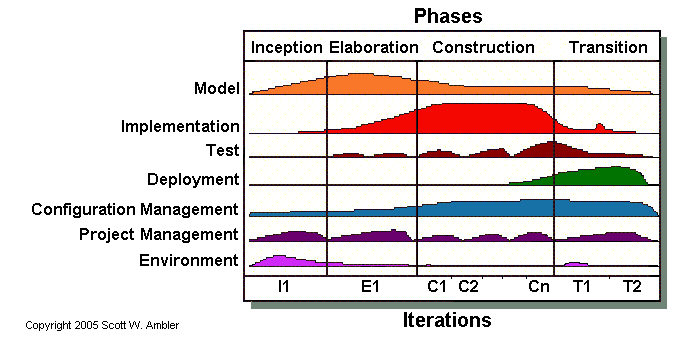
\includegraphics[scale=0.6]{./figuras/lifecycleAgileUP.png}

        \caption{\label{figura:ciclo_AUP}Ciclo de vida da \textit{AUP}. \cite{ProgrammingLanguages}}
    \end{center}
\end{figure}

A natureza serial da AUP é capturada em quatro fases:
\begin{enumerate}
    \item Início: Identificar o escopo inicial do projeto, arquitetura potencial do sistema e obtenção de fundos iniciais advindos dos interessados em seu desenvolvimento.

    \item Elaboração: Discutir a arquitetura do sistema, buscando a prova de que seus conceitos são bons.

    \item Construção: Construir um software funcional, com bases incrementais e regulares, capazes de atender às mais altas prioridades estabelecidas pelos interessados em seu desenvolvimento.

    \item Transição: Validar e implantar o sistema em um ambiente de produção.
\end{enumerate}

Sobre as disciplinas envolvidas, temos sua descrição como:
\begin{itemize}
    \item Modelo: entender as regras de negócio, o domínio que especifica os problemas que devem ser atacados pelo projeto e identificar soluções que os resolvam.

    \item Implementação: transformar o modelo, em código, além de realizar testes básicos, em particular, testes unitários.

    \item Test: realizar avaliações objetivas que garantam a qualidade do software.

    \item Entrega: planejar a entrega do sistema, de modo que seja executado um plano capaz de fazer com que seus usuários finais estejam confortáveis com sua adoção/utilização.

    \item Configuração do Projeto: gerenciar o acesso aos artefatos do projeto, incluindo o rastreamento de suas versões ao longo do tempo e gerenciar mudanças entre si.

    \item Gerenciamento do Projeto: direcionar atividades relacionadas à gerência do projeto, tais como a gerêcia de riscos, delegação de tarefas e manipulação de recursos fora do escopo do desenvolvimento do projeto, para que seja garantida sua entrega.

    \item Ambiente: garantir que os recursos necessários para que seu desenvolvimento e implantação estejam disponíveis ao time de desenvolvimento.
\end{itemize}

\clearpage
\section{Diagramas de Casos de Uso}

Os Diagramas de Casos de Uso foram elaborados, como parte auxiliar do projeto da ferramenta, obedecendo aos requisitos funcionais e não-funcionais, compreendidos por todas as características da ferramenta, previamente apresentadas no capítulo \ref{2_ferramenta_cll}.

O Diagrama de Caso de Uso relativo ao usuário, ilustrado pela figura \ref{figura:uc-usuario}, mostra quais tipos de interação que o usuário pode ter com a ferramenta.

\begin{figure}[ht]
    \begin{center}
        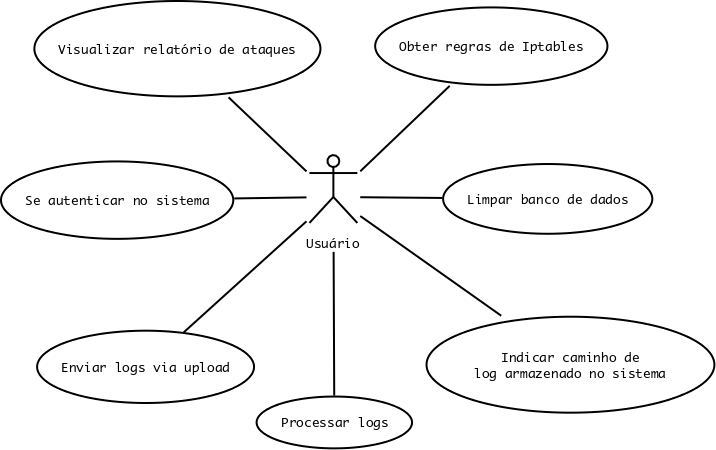
\includegraphics[scale=0.4]{./figuras/uc-usuario.png}

        \caption{\label{figura:uc-usuario}Diagrama de Caso de Uso relativo ao usuário.}
    \end{center}
\end{figure}

\clearpage
Diagrama de Caso de Uso relativo ao \textit{Crickets' little leg}, ilustrado pela figura \ref{figura:uc-ccl}, mostra os requisitos não-funcionais aos quais a ferramenta encontra-se atrelada.

\begin{figure}[ht]
    \begin{center}
        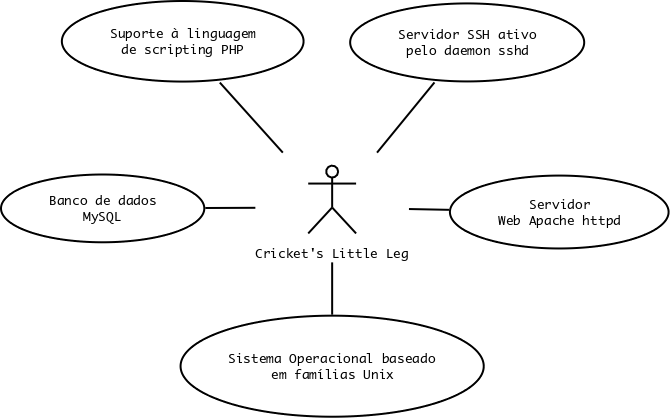
\includegraphics[scale=0.4]{./figuras/uc-ccl.png}

        \caption{\label{figura:uc-ccl}Diagrama de Caso de Uso relativo ao \textit{Crickets' little leg}.}
    \end{center}
\end{figure}

\clearpage
\section{Diagrama de classes}

Seguindo as convenções do design \textit{pattern MVC}, adotado como padrão pelo \textit{framework} de desenvolvimento \textit{CakePHP}, que fora utilizado para o desenvolvimento da ferramenta, foram elaboradas, de acordo com suas categorias enumeradas, as seguintes classes:

\begin{singlespacing}
\begin{enumerate}
    \item Classe de Modelo
        \begin{itemize}
            \item \textit{Entry}
        \end{itemize}
    \item Classes de Controladores
        \begin{itemize}
            \item \textit{EntriesController}
            \item \textit{PagesController}
        \end{itemize}
\end{enumerate}
\end{singlespacing}

Para as classes apresentadas, foi elaborado um Diagrama de Classes, ilustrado pela figura \ref{figura:dc-mvc}, como parte auxiliar no projeto da ferramenta. É importante atentar-se ao fato de que as classes apresentadas, têm como herança, classes advindas do \textit{framework CakePHP}. Desta maneira, tais superclasses tiveram seus atributos e métodos suprimidos no diagrama em questão.

\begin{figure}[hc]
    \begin{center}
        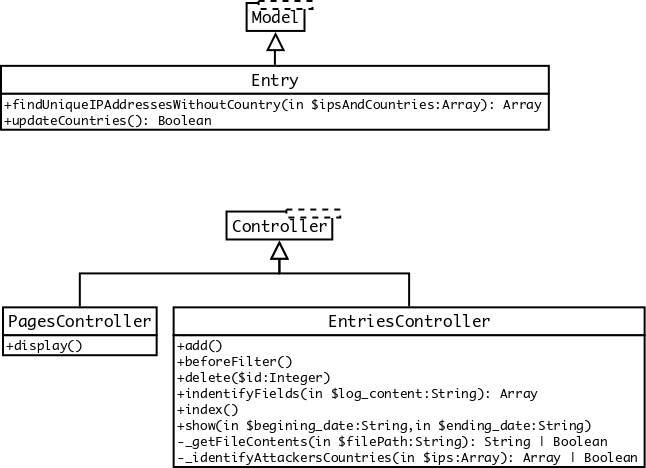
\includegraphics[scale=0.4]{./figuras/dc-mvc.png}

        \caption{\label{figura:dc-mvc}Diagrama de Classes geral do \textit{Crickets' little leg}.}
    \end{center}
\end{figure}

\clearpage
\section{Modelo Entidade Relacionamento}

O banco de dados da ferramenta é muito simples, tendo em vista que os únicos dados armazenados são os resultados das capturas obtidas, através da interpretação dos logs especificados pelo usuário. Todas as entradas, ficam armazenadas em uma tabela, chamada \textit{Entry}. Os países identificados em cada entrada, são armazenados na tabela \textit{Country}. Cada entrada, se relaciona com um país por meio da chave ``country\_id'', presente em \textit{Entry}, sendo correspondida em \textit{Country} por sua chave primária, ou simplesmente ``id''. O Modelo Entidade Relacionamento da ferramenta é ilustrado pela figura \ref{figura:er}:

\begin{figure}[hc]
    \begin{center}
        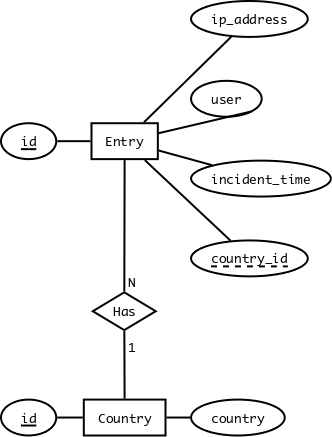
\includegraphics[scale=0.5]{./figuras/er.png}

        \caption{\label{figura:er}Modelo Entidade Relacionamento geral do \textit{Crickets' little leg}.}
    \end{center}
\end{figure}
